\section{Acompanhar Lançamentos}

\subsection{Caso de uso descritivo}

Este caso de uso tem como função permitir que o usuário consiga acompanhar os lançamentos realizados em sua conta.

\begin{table}[h]
  \centering
  \begin{tabular}{|p{4cm} | p{10cm} |}
      \hline
      \small{\textbf{Requisitos Não Funcionais Associados}}	&	Tempo de acesso, segurança, interface amigável e acessível	\\ \hline
      \small{\textbf{Pré-condição}}	&	O usuário deve ser cliente do banco e deve possuir uma conta ativa	\\ \hline
      \small{\textbf{Pós-condição}}	&	O usuário visualiza os lançamentos realizados de acordo com o filtro aplicado	\\ \hline
    \end{tabular}
 \captionof{table}{Condições para o caso de uso Acompanhar Lançamentos}
\end{table}

\textbf{Fluxo de eventos principal:}

\begin{enumerate}
  \item O usuário acessa o sistema utilizando suas credenciais.
  \item O sistema realiza a validação dos dados informados.
  \item O usuário seleciona a opção ``Lançamentos da minha conta''.
  \item O sistema exibe opções de filtros a serem aplicados nos lançamentos.
  \item O usuário seleciona a opção ``Todos os lançamentos''.
  \item O sistema solicita o levantamento dos lançamentos da conta do usuário.
  \item Ao obter os dados dos lançamentos da conta do usuário, o sistema retorna os lançamentos para a tela, informando os lançamentos de acordo com o filtro aplicado.
\end{enumerate}

\textbf{Fluxos secundários:}

\begin{itemize}
  \item \textbf{Fluxo secundário – Acompanhar lançamentos no modo débito}

  No passo 5 do fluxo de eventos principal:
  \subitem Se o usuário selecionar ``Lançamentos no modo débito'', só serão exibidos os lançamentos referentes ao modo débito.

  \item \textbf{Fluxo secundário – Acompanhar lançamentos no modo crédito}

  No passo 5 do fluxo de eventos principal:
  \subitem Se o usuário selecionar ``Lançamentos no modo débito'', só serão exibidos os lançamentos referentes ao modo crédito.
\end{itemize}

\subsection{Diagrama de caso de uso}

\begin{figure}[!htb]
     \centering
     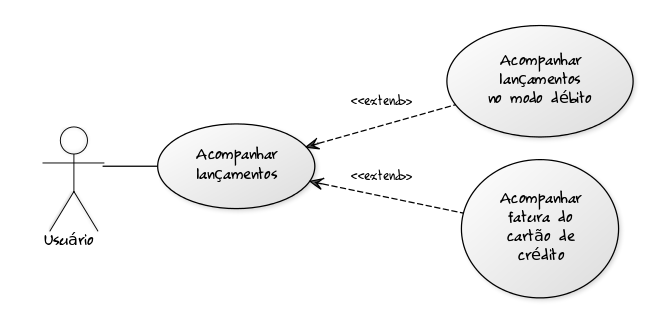
\includegraphics[scale=0.6]{diagramas/caso-de-uso/imagens/acompanharLancamento.png}
     \caption{Caso de uso Acompanhar Lançamento}
\end{figure}

\subsection{Diagrama de classes para o caso de uso}
